\documentclass[11pt]{article}
\usepackage[utf8]{inputenc}
\usepackage[margin=1in]{geometry}
\usepackage{amsmath,amssymb}
\usepackage{graphicx}
\usepackage{booktabs}
\usepackage{float}
\usepackage{setspace}
\usepackage[round]{natbib}
\usepackage[hidelinks]{hyperref}
\onehalfspacing

\title{Concentrated Sectors Connect Less:\\Within-Sector Concentration and Time-Varying Connectedness\\in the S\&P 500, 2018 to 2026}
\author{Tanishk Yadav\thanks{Department of Finance and Risk Engineering, New York University Tandon School of Engineering, New York, NY, USA. Email: \texttt{tanishkyadav@nyu.edu}.}}
\date{October 2026}

\begin{document}
\maketitle

\begin{abstract}
\noindent
The ten largest firms rose from 24\% to 41\% of S\&P 500 market capitalization between 2018 and 2025, and by August 2026 connectedness among the eleven GICS sectors had fallen to its lowest level in the sample. This paper asks whether the two are linked, using daily returns of the Select Sector SPDR funds from October 2018 to August 2026, an uncapped constituent panel with point-in-time membership, and a filtered TVP-VAR. Sector connectedness is contemporaneous: Granger links found by classical tests vanish under heteroskedasticity-robust inference, and directional measures computed from the covariance matrix alone have a correlation of 0.99 with those of the full model. Net directional positions are a product of row normalization. Under a scalar normalization they carry no information, and neither does the effect of concentration on them. What survives is a relationship between concentration and co-movement. On uncapped returns, a one-point rise in a sector's top-three share lowers its monthly $R^2$ against the rest of the market by 0.75 points, and the result holds when concentration paths are randomly reassigned across sectors ($p=0.04$). The three largest firms co-move less with the market than the rest of their sector in 91 of 99 sector-years. Holding their weights at 2018 levels, however, would have raised the system's average squared correlation over the last twelve months only from 10.1\% to 11.0\%. Concentration helps explain which sectors are least connected, not why the market as a whole disconnected.

\medskip
\noindent\textbf{Keywords:} connectedness, market concentration, granularity, normalization, randomization inference, TVP-VAR
\\\noindent\textbf{JEL:} C12, C23, C32, G12, L11
\end{abstract}

\newpage
%============================================================
\section{Introduction}
%============================================================

U.S. equity market concentration is at its highest level in decades. In our constituent panel the ten largest firms held 24\% of S\&P 500 market capitalization at the end of 2018 and 41\% at the end of 2025. Within sectors it is higher still: by August 2026 the three largest firms held 82\% of Communication Services and 54\% of Information Technology, against 18\% of Industrials.

Over the same years the eleven sectors of the index drifted apart. Total connectedness among them, in the sense of \citet{diebold2012}, peaked in the COVID-19 crash and reached the lowest value of our sample in August 2026. A common reading of concentration is that it makes the market more fragile, because a shock to one giant firm moves everything. The sector-level data suggest something closer to the opposite. A separate literature, following \citet{gabaix2011}, argues that when a few firms are large relative to their aggregate, their idiosyncratic shocks no longer diversify away. Applied one level down, the argument predicts that a sector whose return is driven by two or three firms will look idiosyncratic to the other sectors. The connectedness and granularity literatures have not met, and this paper brings them together.

The sample covers the eleven GICS sectors from October 2018 to August 2026, a window that contains the late-2018 sell-off, the COVID-19 crash, the 2022 rate shock, the March 2023 regional bank failures, and the April 2025 tariff shock. Sector returns come from the Select Sector SPDR funds, which track the full GICS sectors with point-in-time membership. Concentration comes from a separate constituent panel that uses point-in-time index membership, historical share counts, and the March 2023 GICS reclassification. Time variation comes from a TVP-VAR estimated by a forgetting-factor Kalman filter \citep{koop2013, antonakakis2020}, so each daily estimate uses only data available that day. A firm-level decomposition then splits every sector's return into the return on its three largest firms and the return on the rest of the sector.

The paper makes three contributions.

The first concerns what daily sector connectedness measures. Pairwise Granger tests with classical F statistics find 90 of 110 directed links significant after false-discovery-rate control. The tests are oversized under GARCH errors, heteroskedasticity-robust tests leave no link standing, and the classical rejections come almost entirely from February to June 2020, when all sectors reversed together from one day to the next. Lagged cross-sector returns have negative out-of-sample $R^2$ for every sector. Because lags carry so little, the directional measures are a transformation of the correlation matrix: computed from the covariance matrix alone, net directional connectedness has a correlation of 0.99 with the full model. The transformation is not neutral. Row normalization compresses what a sector receives into a narrow band and lets what it transmits vary widely, so a sector whose correlations with everyone fall becomes a ``net receiver.'' Under the scalar normalization proposed by \citet{caloia2019}, net positions are close to zero for every sector. These points apply to any connectedness study built on daily equity returns.

The second is a filtered, daily history of return and volatility connectedness through August 2026. Total return connectedness peaked at 88.9\% on 16 March 2020 and reached its sample low of 53.7\% in late August 2026. The decline in 2026 is broad: average pairwise correlation among the funds fell from 0.58 in 2025 to 0.21 in the first eight months of 2026, and Information Technology moved against the rest of the market from May to August. A 200-day rolling window, the default in applied work, understates the April 2025 jump and then drops by more than 20 points when the shock leaves the window.

The third is the link between concentration and co-movement, estimated with inference built for slow-moving regressors. Monthly connectedness from the filter and within-sector concentration both behave almost like sector-specific trends, and a panel of one on the other produces large Driscoll-Kraay $t$-statistics that a permutation test shows to be unremarkable. Measures of co-movement computed afresh each month are far less persistent. On uncapped constituent returns they fall with concentration, and the relationship survives randomization inference. The firm-level decomposition shows why: the three largest firms co-move less with the market than the rest of their sector in 91 of 99 sector-years. It also bounds the effect. Holding the top-three weights at their 2018 levels changes the system's average squared correlation in the last twelve months by less than one point, against a fall of 28 points since 2018.

The rest of the paper is organized as follows. Section~\ref{sec:lit} places the paper in the literature. Section~\ref{sec:data} describes the data. Section~\ref{sec:method} sets out the econometrics. Section~\ref{sec:results} reports results, and Section~\ref{sec:disc} discusses the results that run against intuition.

%============================================================
\section{Related literature}\label{sec:lit}
%============================================================

\textbf{Connectedness.} \citet{diebold2009} measure spillovers with forecast-error variance decompositions from a VAR; \citet{diebold2012} replace the Cholesky decomposition with the order-invariant generalized decomposition of \citet{koop1996} and \citet{pesaran1998}, which also yields directional measures; \citet{diebold2014} link the measures to network degree. \citet{antonakakis2020} replace the rolling window with a TVP-VAR estimated by the forgetting-factor Kalman filter of \citet{koop2013}, and \citet{barunik2018} decompose connectedness by frequency. \citet{billio2012} measure system-wide linkages among financial institutions with principal components and Granger networks. Two papers question how the generalized decomposition is normalized. \citet{caloia2019} show that row normalization can produce net spillovers of the wrong sign and rank, and recommend dividing by the largest row sum. \citet{lastrapes2021} propose a joint spillover index and find, on U.S. industry returns, that it can differ substantially from the generalized one.

\textbf{Cross-industry predictability and daily reversals.} A lead-lag literature argues that information diffuses slowly across economically linked industries: \citet{hou2007} finds that large firms lead small firms within industries, \citet{menzly2010} document cross-predictability along supply chains at monthly frequency, and \citet{hong2007} report that some industries lead the aggregate market. \citet{rapach2019} find out-of-sample industry predictability at monthly frequency. \citet{vilasuso2001} shows that causality tests are unreliable under conditional heteroskedasticity. At the daily horizon, price moves driven by liquidity demand tend to reverse \citep{campbell1993}, the returns to supplying that liquidity rise sharply with the VIX \citep{nagel2012}, and the growth of index products has made daily index returns negatively autocorrelated \citep{baltussen2019}.

\textbf{Concentration and granularity.} \citet{gabaix2011} shows that when the firm-size distribution is fat-tailed, idiosyncratic shocks to large firms generate aggregate fluctuations. \citet{grullon2019} and \citet{kwon2024} document rising concentration across U.S. industries. \citet{campbell2001} show that idiosyncratic volatility is a large and time-varying part of stock risk. To our knowledge, no study relates within-sector concentration to a sector's position in the connectedness network.

\textbf{Inference with persistent regressors.} \citet{ferson2003} show that regressions involving persistent financial series produce spurious significance even in large samples. With few clusters, \citet{cameron2008} and \citet{webb2023} recommend the wild cluster bootstrap, and \citet{young2019} shows how often randomization tests overturn conventional significance.

%============================================================
\section{Data}\label{sec:data}
%============================================================

\subsection{Sector returns and volatility}

Sector returns are daily log returns, in percent, of the eleven Select Sector SPDR funds (XLC, XLY, XLP, XLE, XLF, XLV, XLI, XLK, XLB, XLRE, XLU), adjusted for distributions. The sample runs from 1 October 2018 to 31 August 2026, 1,989 trading days. The start date follows the September 2018 GICS reorganization that created Communication Services. The funds cover every member of each sector, their membership is point-in-time, and they are investable. Their disadvantage is weight capping, which limits single-name weights and therefore understates concentration where it is highest. We address this with a second return series built from constituents without caps (Section~\ref{sec:const}).

Volatility is the \citet{parkinson1980} range estimator, $\hat\sigma^2_t = (\ln H_t - \ln L_t)^2/(4\ln 2)$, annualized and in logs, $v_t = \ln(100\sqrt{252\,\hat\sigma^2_t})$. Table~\ref{tab:desc} reports summary statistics. Every sector has negative skewness and excess kurtosis between 7 and 17. Log volatility is persistent, with first-order autocorrelation between 0.50 and 0.63.

\subsection{Constituents, market capitalization, and concentration}\label{sec:const}

Index membership is point-in-time: current members enter on their S\&P 500 addition date, and firms removed during the sample enter and leave on their actual dates. Removed firms are kept when price and share data remain available, which recovers 78 firms; firms that were acquired and delisted cannot be recovered. A removed ticker whose price path duplicates a current ticker is treated as a rename rather than a second firm. The panel covers 428 firms on the first day and 497 on the last.

Market capitalization is the daily closing price times historical shares outstanding, with both series on the same split basis and a five-day rolling median applied to the vendor share series to remove recording spikes. Firms with two listed share classes are counted once. Firms are assigned to GICS sectors with the March 2023 reclassification applied on its effective date: payment processors are in Information Technology before 17 March 2023 and in Financials after, and Target, Dollar General, and Dollar Tree move from Consumer Discretionary to Consumer Staples on the same date.

For sector $s$ on day $t$, with market-capitalization weights $w_{i,t}$ inside the sector, the two concentration measures are the Herfindahl index $\text{HHI}_{s,t} = \sum_i w_{i,t}^2$ and the top-three share, the sum of the three largest weights. Both use total rather than float-adjusted market capitalization, which is the economically relevant size for the granular argument. The index-level top-ten share computed this way is 24.1\% at the end of 2018, 33.0\% at the end of 2023, and 40.8\% at the end of 2025, within one to three points of published float-adjusted figures.

Figure~\ref{fig:conc} shows the top-three share by sector. Concentration rose most in Communication Services (62\% to 82\%), Consumer Discretionary (48\% to 65\%), Information Technology (45\% to 55\%), and Consumer Staples (38\% to 49\%), and fell slightly in Industrials, Financials, and Energy.

A second, uncapped return series weights each constituent's daily return by its previous-day market capitalization inside its sector. Its daily correlation with the corresponding fund is between 0.986 and 0.999 for ten sectors and 0.926 for Communication Services, where fund caps bind hardest.

\subsection{The three largest firms}\label{sec:firms}

For the firm-level decomposition we collect the same price and share data for 121 firms that could hold a top-three position in some sector during the sample, between 9 and 15 per sector. On every day after 6 November 2018 the top-three share computed from these candidates equals the share from the full panel in nine sectors and is within two points in Industrials and Materials. Before that date Praxair, which left the index in the Linde merger and is not among the candidates, was one of the three largest Materials firms; the decomposition's base period therefore starts on 6 November 2018.

\begin{table}[H]
\centering
\caption{Summary statistics, 1 October 2018 to 31 August 2026 (1,989 days)}
\label{tab:desc}
\small
\begin{tabular}{lrrrrrrrr}
\toprule
& \multicolumn{4}{c}{Daily log return} & \multicolumn{2}{c}{Log range volatility} & \multicolumn{2}{c}{Top-3 share (\%)} \\
\cmidrule(lr){2-5}\cmidrule(lr){6-7}\cmidrule(lr){8-9}
Sector & Mean & Vol. & Skew & Ex. kurt. & Mean & AR(1) & 2018Q4 & 2026 \\
\midrule
Communication Services & 11.4 & 22.4 & $-0.47$ & 7.1 & 2.54 & 0.57 & 62.1 & 82.3 \\
Consumer Discretionary & 9.6 & 24.3 & $-0.51$ & 7.3 & 2.61 & 0.63 & 47.7 & 65.4 \\
Consumer Staples & 8.4 & 15.8 & $-0.42$ & 14.3 & 2.29 & 0.53 & 38.3 & 49.2 \\
Energy & 11.0 & 32.4 & $-0.95$ & 14.9 & 2.92 & 0.58 & 54.7 & 54.0 \\
Financials & 11.2 & 23.6 & $-0.58$ & 15.5 & 2.53 & 0.58 & 35.8 & 31.0 \\
Health Care & 9.1 & 17.7 & $-0.33$ & 9.5 & 2.40 & 0.50 & 27.7 & 33.4 \\
Industrials & 11.8 & 21.6 & $-0.48$ & 12.6 & 2.49 & 0.58 & 19.4 & 17.9 \\
Information Technology & 21.2 & 27.2 & $-0.26$ & 7.5 & 2.69 & 0.55 & 44.7 & 54.8 \\
Materials & 9.6 & 22.2 & $-0.40$ & 9.3 & 2.55 & 0.55 & 36.6 & 36.9 \\
Real Estate & 7.1 & 22.2 & $-1.04$ & 17.4 & 2.59 & 0.51 & 27.5 & 32.0 \\
Utilities & 9.0 & 20.6 & $-0.25$ & 15.0 & 2.59 & 0.50 & 27.6 & 27.9 \\
\bottomrule
\end{tabular}

\smallskip
\parbox{0.95\textwidth}{\footnotesize Mean and volatility of returns are annualized, in percent. Log range volatility is the log of the annualized Parkinson volatility in percent. The top-three share is the average of daily values over October to December 2018 and over January to August 2026.}
\end{table}

\begin{figure}[H]
\centering
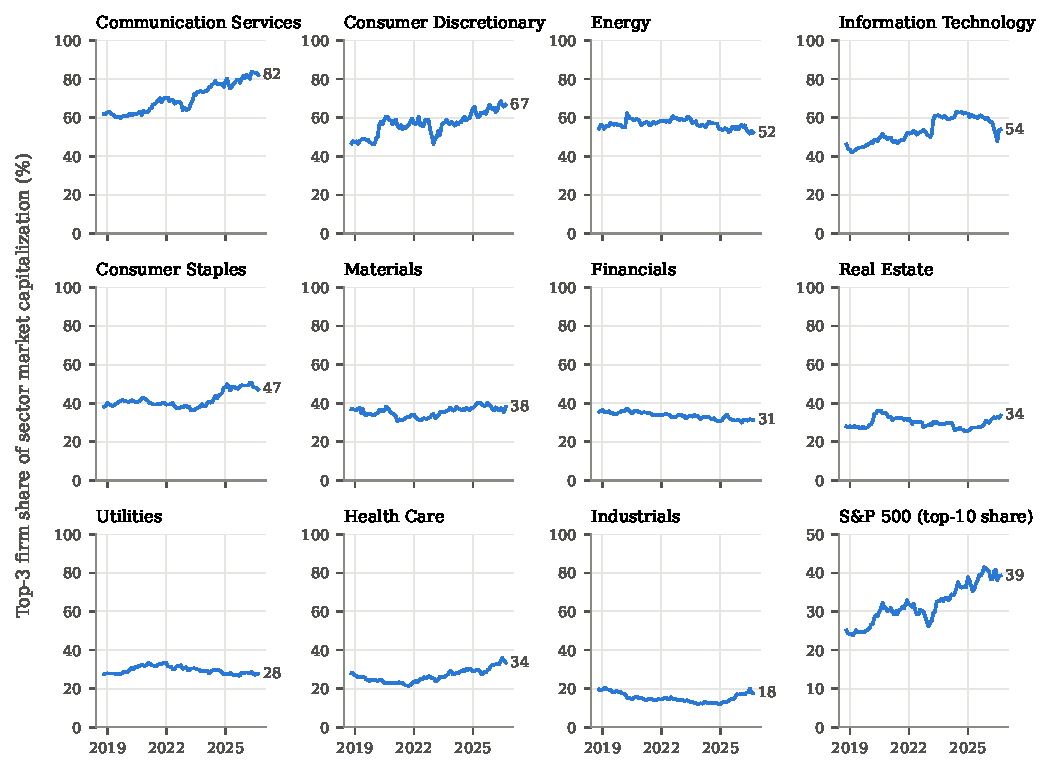
\includegraphics[width=\textwidth]{fig/fig2_concentration.pdf}
\caption{Share of sector market capitalization held by the three largest firms, month-end, October 2018 to August 2026. The last panel is the top-ten share of the whole index. Values at the right edge are August 2026.}
\label{fig:conc}
\end{figure}

%============================================================
\section{Methodology}\label{sec:method}
%============================================================

\subsection{Generalized connectedness and its normalization}

Let $y_t$ be the $k=11$ vector of sector returns (or log volatilities), with VAR($p$) representation $y_t = c + \sum_{l=1}^{p} B_l y_{t-l} + u_t$, $u_t \sim (0,\Sigma)$, and moving-average coefficients $\Phi_h$. The generalized forecast-error variance decomposition of \citet{pesaran1998} at horizon $H$ is
\begin{equation}
\theta_{ij}(H) = \frac{\sigma_{jj}^{-1}\sum_{h=0}^{H-1}\left(e_i'\Phi_h\Sigma e_j\right)^2}{\sum_{h=0}^{H-1} e_i'\Phi_h\Sigma\Phi_h' e_i},
\qquad \tilde\theta_{ij}(H) = \frac{\theta_{ij}(H)}{\sum_{j}\theta_{ij}(H)},
\end{equation}
the share of sector $i$'s $H$-step forecast-error variance attributable to shocks in sector $j$. Following \citet{diebold2012}, in percent,
\begin{equation}
\text{FROM}_i = \sum_{j\neq i}\tilde\theta_{ij}, \quad \text{TO}_j = \sum_{i\neq j}\tilde\theta_{ij}, \quad \text{NET}_i = \text{TO}_i - \text{FROM}_i, \quad \text{TCI} = \frac{1}{k}\sum_{i\neq j}\tilde\theta_{ij}.
\end{equation}
We set $H=10$ and choose $p$ by BIC. For daily returns BIC selects no lags and we use $p=1$; for log volatility it selects $p=1$.

The row normalization $\tilde\theta$ divides each row by its own sum, so FROM is bounded by 100 while TO is not. \citet{caloia2019} instead divide every element of $\theta$ by the largest row sum, a single scalar that preserves magnitudes across rows; we report both. A useful benchmark is the case with no lag dynamics. When $\Phi_h=0$ for $h\geq 1$, $\theta_{ij} = \rho_{ij}^2$, the squared correlation between the two sectors' innovations. The row-normalized measures are then functions of the correlation matrix alone,
\begin{equation}
\text{FROM}_i = 100\left(1-\frac{1}{S_i}\right), \qquad \text{TO}_j = 100\sum_{i\neq j}\frac{\rho_{ij}^2}{S_i}, \qquad S_i=\sum_{k}\rho_{ik}^2,
\end{equation}
and under the scalar normalization the matrix is symmetric, so TO equals FROM and NET is zero for every sector. We compute this covariance-only version, with $H=1$, alongside the full model.

\subsection{Time-varying parameter VAR}

The TVP-VAR is $y_t = Z_t\beta_t + u_t$ with $Z_t = I_k\otimes(1, y_{t-1}')$, $\beta_t = \beta_{t-1}+\xi_t$, and $u_t\sim(0,\Sigma_t)$. Following \citet{koop2013} and \citet{antonakakis2020}, the state covariance is inflated by a forgetting factor rather than estimated, $P_{t|t-1} = P_{t-1|t-1}/\kappa_1$, and the measurement covariance is an exponentially weighted average of prediction errors, $\Sigma_t = \kappa_2\Sigma_{t-1}+(1-\kappa_2)\hat u_t\hat u_t'$, with $\kappa_1=\kappa_2=0.99$. The intercept is included because log volatility has a large mean. The filter starts on 20 June 2018 with $\beta_0=0$ and $P_0 = 0.1I$, and estimates before 1 October 2018 are discarded as burn-in. We use filtered, not smoothed, estimates, so the measure on day $t$ uses only data through day $t$. At each date the measures in (2) are computed from $(\beta_{t|t},\Sigma_t)$ under both normalizations, and from $\Sigma_t$ alone.

\subsection{Granger causality and out-of-sample predictability}

For each ordered pair $(j, i)$ we test whether lags of $y_j$ enter the equation for $y_i$. The system version conditions on the lags of all eleven sectors; the bivariate version conditions only on lags of $y_i$. Test statistics are Wald statistics with the HC3 covariance estimator, which is valid under conditional heteroskedasticity of unknown form. For comparison we also report classical F statistics. Across the 110 ordered pairs, $p$-values are adjusted with the \citet{benjamini1995} false-discovery-rate procedure and with Bonferroni.

For each sector we forecast the next day's return from the current returns of all eleven sectors, re-estimating by OLS on an expanding window that starts with the first quarter of the sample, so the evaluation period begins on 23 September 2020. We also report the equal-weighted combination of eleven single-predictor forecasts. The benchmark is the prevailing historical mean. We report $R^2_{OS} = 1 - \sum(r - \hat r)^2/\sum(r-\bar r)^2$ \citep{campbell2008} and the \citet{clark2007} test with Newey-West variance.

\subsection{Concentration and co-movement}

The baseline panel regression is
\begin{equation}
C_{s,m} = \alpha_s + \delta_m + \gamma\,\text{Conc}_{s,m-1} + \phi_1\ln(\text{share}_{s,m-1}) + \phi_2 \bar v_{s,m} + \varepsilon_{s,m},
\end{equation}
where Conc is the top-three share or the HHI in percentage points, share is the sector's weight in the index, and $\bar v$ is the sector's average log volatility in the period. Sector fixed effects remove permanent differences between sectors, and period fixed effects remove anything common to all sectors, including the level of system connectedness and market volatility. The monthly panel has 11 sectors and 94 months, November 2018 to August 2026.

We use two kinds of outcome $C$. The first is the monthly average of daily TVP-VAR FROM, TO, and NET, under each normalization. The second is measured afresh in each period from that period's daily returns only: the $R^2$ of the sector's return on the equal-weighted return of the other ten sectors, and the average squared correlation with each of the other ten, $\bar\rho^2_s$. We compute both monthly (1,034 observations) and quarterly (341).

The two kinds of outcome call for different care. Monthly averages of the filtered measures inherit the filter's memory, an effective window of about 100 trading days. Concentration is also persistent: its within-sector first-order autocorrelation is 0.94, and sector-specific linear trends absorb 59\% of its within-sector variation after the fixed effects. Regressing one slow-moving series on another can yield large $t$-statistics without any relationship \citep{ferson2003}. We therefore report three kinds of inference for $\gamma$: \citet{driscoll1998} standard errors with three lags; sector-clustered standard errors with $p$-values from the wild cluster restricted bootstrap with the six-point weights of \citet{webb2023}, 4,999 draws; and a permutation test. The permutation test reassigns each sector's concentration path to another sector, keeping the controls with their own sector, and recomputes the Driscoll-Kraay $t$-statistic over 2,000 random permutations. It asks whether the observed pairing of concentration and outcome is unusual among all pairings, which is the relevant question when both series trend. Finally, we compare long differences across the eleven sectors: the change in each variable from the first twelve months of the sample to the last twelve.

\subsection{Granular decomposition}

Let $W_{s,t-1}$ be the combined weight of sector $s$'s three largest firms at the close of day $t-1$, with the three chosen on that day's weights. The uncapped sector return splits exactly into
\begin{equation}
r_{s,t} = W_{s,t-1}\, r^{\text{top}}_{s,t} + (1-W_{s,t-1})\, r^{\text{rest}}_{s,t},
\end{equation}
where $r^{\text{top}}$ is the weighted return of the three firms and $r^{\text{rest}}$ follows from the identity. We measure each component's co-movement with the equal-weighted return of the other ten sectors. The counterfactual return holds the weight at its average from 6 November to 31 December 2018, $r^{\text{cf}}_{s,t} = \bar W_s\, r^{\text{top}}_{s,t} + (1-\bar W_s)\, r^{\text{rest}}_{s,t}$. The comparison is accounting, not regression. It keeps the component returns as they were, so it measures how much the shift in weight alone changed co-movement.

%============================================================
\section{Results}\label{sec:results}
%============================================================

\subsection{Static connectedness}

Over the full sample the total connectedness index is 79.5\% for returns and 77.7\% for volatility (Table~\ref{tab:static}). Industrials has the largest NET in both systems, followed by Materials and Financials for returns. Energy has the most negative NET for returns and Utilities for volatility.

The return index barely moves with the VAR specification: across lag orders 1, 2, and 5 and horizons 5, 10, and 20 it ranges from 79.4\% to 79.5\%, and from 78.6\% to 78.7\% on the uncapped constituent series. The covariance matrix alone gives 79.7\%. The eleven NET values from the covariance matrix have a correlation of 0.998 with those in Table~\ref{tab:static} and never differ from them by more than 1.3 points. Return connectedness is almost entirely contemporaneous correlation, and Section~\ref{sec:granger} confirms this directly. Volatility connectedness, where lagged dynamics matter, ranges from 72.6\% to 77.7\%.

\begin{table}[H]
\centering
\caption{Static connectedness, full sample}
\label{tab:static}
\small
\begin{tabular}{lrrrrrrrr}
\toprule
& \multicolumn{4}{c}{Returns} & \multicolumn{4}{c}{Log range volatility} \\
\cmidrule(lr){2-5}\cmidrule(lr){6-9}
Sector & Own & FROM & TO & NET & Own & FROM & TO & NET \\
\midrule
Communication Services & 20.2 & 79.8 & 76.5 & $-3.3$ & 20.8 & 79.2 & 85.7 & 6.5 \\
Consumer Discretionary & 18.6 & 81.4 & 84.7 & 3.3 & 21.9 & 78.1 & 90.6 & 12.4 \\
Consumer Staples & 22.0 & 78.0 & 72.1 & $-5.9$ & 21.7 & 78.3 & 77.5 & $-0.8$ \\
Energy & 28.8 & 71.2 & 46.0 & $-25.2$ & 26.8 & 73.2 & 52.6 & $-20.6$ \\
Financials & 17.3 & 82.7 & 97.2 & 14.5 & 20.6 & 79.4 & 86.7 & 7.3 \\
Health Care & 20.2 & 79.8 & 80.5 & 0.6 & 22.8 & 77.2 & 67.7 & $-9.5$ \\
Industrials & 16.2 & 83.8 & 103.6 & 19.8 & 19.4 & 80.6 & 99.5 & 18.9 \\
Information Technology & 20.6 & 79.4 & 73.1 & $-6.3$ & 21.4 & 78.6 & 83.0 & 4.5 \\
Materials & 17.0 & 83.0 & 97.5 & 14.5 & 19.8 & 80.2 & 94.7 & 14.5 \\
Real Estate & 19.4 & 80.6 & 83.4 & 2.8 & 24.7 & 75.3 & 63.4 & $-11.8$ \\
Utilities & 24.8 & 75.2 & 60.3 & $-15.0$ & 25.4 & 74.6 & 53.2 & $-21.4$ \\
\midrule
TCI & \multicolumn{4}{r}{79.5} & \multicolumn{4}{r}{77.7} \\
\bottomrule
\end{tabular}

\smallskip
\parbox{0.95\textwidth}{\footnotesize Generalized variance decomposition at $H=10$ from a VAR(1), row normalization, in percent. Own is the diagonal share.}
\end{table}

\subsection{Time-varying connectedness}

Figure~\ref{fig:tci} plots the filtered TCI. Return connectedness averages 75.4\%. It rises through the fourth quarter of 2018, jumps to its sample maximum of 88.9\% on 16 March 2020, decays through 2021, rises again during the 2022 rate shock, and jumps by roughly 15 points in the first days of April 2025. From late 2025 it falls steadily, to 53.7\% on 26 August 2026, the lowest value in the sample. Volatility connectedness follows the same path, peaking at 86.9\% on 25 March 2020 and reaching its low of 55.5\% on 24 August 2026. Estimates in the first weeks of the sample partly reflect filter initialization and are read with caution.

The 2026 decline is not confined to one sector. The average pairwise correlation of daily fund returns is 0.58 in 2025 and 0.21 from January to August 2026. From May to August 2026 it is 0.14, or 0.20 without Information Technology, whose correlation with the equal-weighted return of the other ten sectors over those four months is $-0.16$. Lagged cross-correlations stay near zero throughout, so the decline is not an artifact of misaligned dates.

The 200-day rolling index in panel (a) shows why the filter matters. After the April 2025 shock the rolling estimate rises to about 77\%, five points below the filtered estimate, stays there until early 2026, and then drops by more than 20 points within a few days. That drop is the tariff shock leaving the window, not a change in the market on those days. The filtered return index is insensitive to the forgetting factors: its correlation with the baseline is 0.999 or higher for $\kappa_1\in\{0.98, 0.995\}$ and 0.79 when the covariance forgetting factor is lowered to 0.96, which makes $\Sigma_t$ noisier. Its correlation with the same estimate on uncapped constituent returns is 0.993.

\begin{figure}[H]
\centering
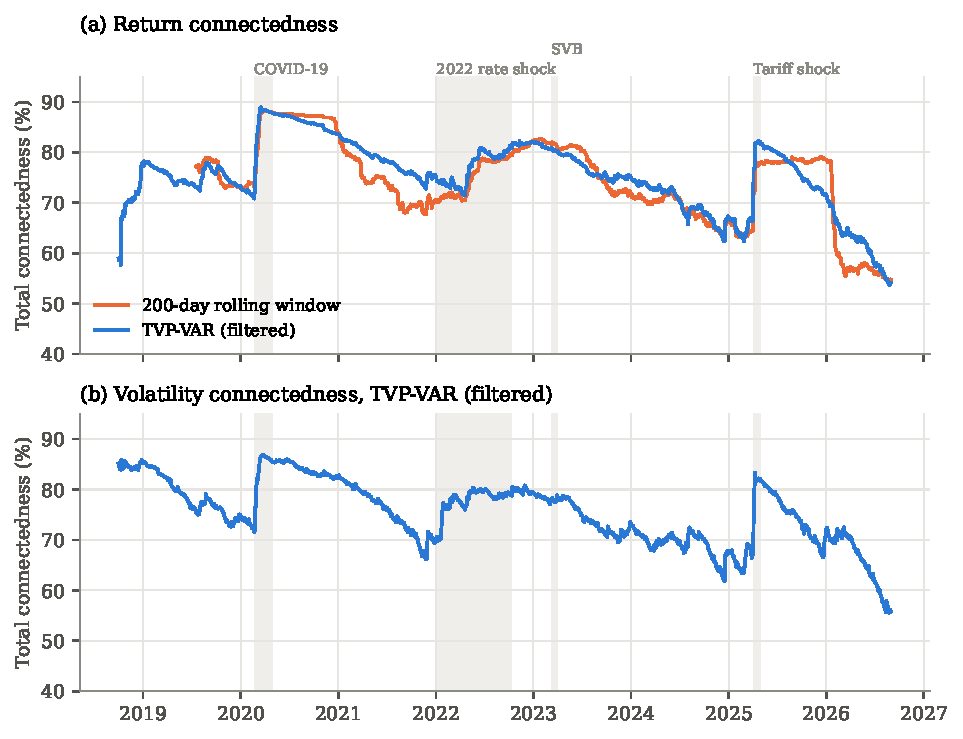
\includegraphics[width=\textwidth]{fig/fig1_tci.pdf}
\caption{Total connectedness index, daily. Panel (a): returns, filtered TVP-VAR and a 200-day rolling VAR. Panel (b): log range volatility, filtered TVP-VAR. Shaded: COVID-19 crash, 2022 rate shock, March 2023 bank failures, April 2025 tariff shock.}
\label{fig:tci}
\end{figure}

\subsection{Lead-lag relationships}\label{sec:granger}

Table~\ref{tab:granger} reports Granger tests across the 110 ordered pairs. Rows (1) to (4) use classical statistics. Taking the minimum $p$-value over lags one to five for each pair, a procedure that is common in applied work, gives 94 raw rejections and 90 after FDR control. Fixing the lag at five reduces this to 77, fixing it at one to 48, and conditioning on the full system to 20. Rows (5) to (7) use HC3 Wald statistics. No link survives FDR control, in the bivariate or system form, at lag one or five, in the full sample or either half.

\begin{table}[H]
\centering
\caption{Granger causality among 110 ordered sector pairs, daily returns}
\label{tab:granger}
\small
\begin{tabular}{llrrr}
\toprule
& Test & Raw $p<0.05$ & FDR & Bonferroni \\
\midrule
\multicolumn{5}{l}{\textit{Full sample, classical statistics}} \\
(1) & Bivariate F, minimum $p$ over lags 1 to 5 & 94 & 90 & \\
(2) & Bivariate F, lag 5 & 80 & 77 & \\
(3) & Bivariate F, lag 1 & 65 & 48 & \\
(4) & System VAR(1), Wald & 40 & 20 & \\
\multicolumn{5}{l}{\textit{Full sample, HC3 Wald}} \\
(5) & Bivariate, lag 1 & 20 & 0 & 0 \\
(6) & Bivariate, lag 5 & 20 & 0 & 0 \\
(7) & System VAR(1) & 6 & 0 & 0 \\
\multicolumn{5}{l}{\textit{Subsamples}} \\
(8) & System VAR(1), HC3, Oct 2018 to Aug 2022 & 15 & 0 & 0 \\
(9) & System VAR(1), HC3, Sep 2022 to Aug 2026 & 4 & 0 & 0 \\
(10) & As (1), excluding 20 Feb to 30 Jun 2020 & 22 & 0 & \\
(11) & As (1), 2021 to 2026 & 12 & 0 & \\
(12) & As (1), calendar 2020 only & 89 & 87 & \\
\bottomrule
\end{tabular}

\smallskip
\parbox{0.95\textwidth}{\footnotesize About 5.5 raw rejections are expected by chance at the 5\% level. FDR is \citet{benjamini1995} at 5\%.}
\end{table}

A Monte Carlo experiment explains the gap. We simulate returns from a one-factor model in which the factor and each sector's residual follow GARCH(1,1) processes with Student-$t$ innovations, all estimated on the fund returns, and in which no sector's lag predicts any other sector. The factor process is highly persistent ($\hat\alpha=0.159$, $\hat\beta=0.815$, $\hat\nu=7.1$). With 1,989 observations and 1,000 replications, the classical F-test at lag five rejects a true null 21.0\% of the time at a nominal 5\%, and the minimum-over-lags procedure rejects 30.7\% of the time. HC3 tests reject 5.2\% (lag one) and 4.1\% (lag five). Over 100 replications of the full 110-pair procedure, the classical minimum-over-lags approach produces 5.3 false FDR survivors on average, with 16.5 at the 90th percentile; HC3 produces 0.09.

The simulation produces far fewer false survivors than the 90 found in the data, so heteroskedasticity inflates the classical test but does not by itself account for the count. Rows (10) to (12) of Table~\ref{tab:granger} locate the rest. Excluding 20 February to 30 June 2020, 4.6\% of trading days, removes every classical FDR survivor, while calendar 2020 alone produces 87. That window contains 97.6\% of the lag-one cross-covariance between sectors over the whole sample. Inside it, the average lag-one correlation between one sector's return and another's is $-0.29$, almost equal to the average own-lag correlation of $-0.28$. Each sector's lagged return predicts the others only because all sectors reversed together from one day to the next, and even within the window no link survives HC3 testing with FDR control.

Out of sample, the lagged returns of other sectors carry no usable information (Table~\ref{tab:oos}). $R^2_{OS}$ is negative for all eleven sectors, between $-4.0\%$ and $-8.8\%$ for the unrestricted regression and between $-0.1\%$ and $-1.9\%$ for the combination forecast. One of 22 Clark-West tests rejects at 5\% and none after FDR control.

\begin{table}[H]
\centering
\caption{Out-of-sample predictability of next-day sector returns, 23 September 2020 to 31 August 2026}
\label{tab:oos}
\small
\begin{tabular}{lrrrr}
\toprule
& \multicolumn{2}{c}{All 11 lagged returns} & \multicolumn{2}{c}{Combination of 11 forecasts} \\
\cmidrule(lr){2-3}\cmidrule(lr){4-5}
Sector & $R^2_{OS}$ (\%) & CW $p$ & $R^2_{OS}$ (\%) & CW $p$ \\
\midrule
Communication Services & $-5.63$ & 0.42 & $-0.95$ & 0.33 \\
Consumer Discretionary & $-5.23$ & 0.55 & $-0.59$ & 0.37 \\
Consumer Staples & $-5.78$ & 0.60 & $-1.87$ & 0.76 \\
Energy & $-4.02$ & 0.03 & $-0.14$ & 0.21 \\
Financials & $-8.83$ & 0.13 & $-1.65$ & 0.65 \\
Health Care & $-7.53$ & 0.47 & $-1.48$ & 0.79 \\
Industrials & $-8.09$ & 0.45 & $-0.81$ & 0.44 \\
Information Technology & $-4.99$ & 0.23 & $-0.72$ & 0.11 \\
Materials & $-6.19$ & 0.32 & $-0.75$ & 0.42 \\
Real Estate & $-6.97$ & 0.44 & $-1.38$ & 0.73 \\
Utilities & $-7.79$ & 0.93 & $-1.19$ & 0.71 \\
\bottomrule
\end{tabular}

\smallskip
\parbox{0.95\textwidth}{\footnotesize Expanding-window OLS; benchmark is the prevailing mean. CW is the one-sided \citet{clark2007} test.}
\end{table}

\subsection{What the directional measures record}\label{sec:norm}

Because lags carry almost no information, the directional measures are in effect a transformation of the correlation matrix. Figure~\ref{fig:norm}(a) compares monthly NET from the TVP-VAR with NET computed from the filtered covariance matrix alone; the correlation is 0.99.

The transformation is not neutral. Under row normalization, FROM is $100(1-1/S_i)$, and for these sectors $S_i$ lies between 3.5 and 6.2, so FROM is confined to a narrow band, 71.2 to 83.8 in Table~\ref{tab:static}. TO sums ten entries that are each divided by a different row sum, and it ranges from 46.0 to 103.6. If one sector's correlations with all others fall by the same proportion, its TO falls 4.5 times as much as its FROM (the median across sectors; the range is 2.1 to 6.8), and its NET falls with it. A sector that becomes less correlated with everyone is labeled a net receiver, whatever the direction of any shock. Under the scalar normalization of \citet{caloia2019}, the full-model NET is close to zero for every sector and has a correlation of 0.11 with the row-normalized NET (Figure~\ref{fig:norm}(b)).

\begin{figure}[H]
\centering
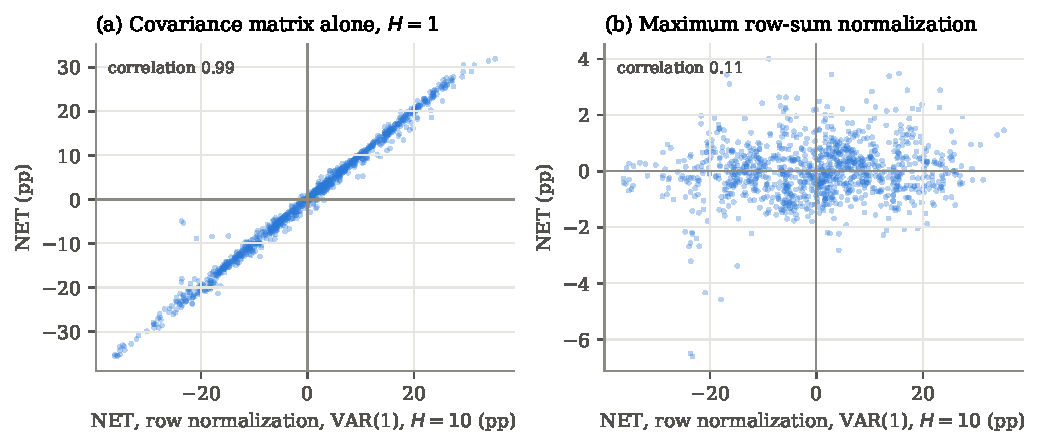
\includegraphics[width=\textwidth]{fig/fig3_normalization.pdf}
\caption{Net directional return connectedness, monthly means of daily filtered estimates, 11 sectors by 94 months. Horizontal axis: TVP-VAR(1), $H=10$, row normalization. Panel (a): row normalization of the filtered covariance matrix alone. Panel (b): the full model under the maximum row-sum normalization of \citet{caloia2019}.}
\label{fig:norm}
\end{figure}

Table~\ref{tab:norm} shows what this does to the effect of concentration. Under row normalization, the top-three share lowers TO and NET but barely moves FROM, the pattern the arithmetic above predicts for a fall in correlation, and the covariance-only measures give the same coefficients. Under the scalar normalization, the effect on NET disappears ($-0.02$, $t=-0.7$, on fund returns), while TO and FROM fall by similar amounts. Concentrated sectors are not net receivers in any meaningful sense. They are less connected in both directions.

\begin{table}[H]
\centering
\caption{Top-three share and connectedness under three versions of the decomposition}
\label{tab:norm}
\small
\begin{tabular}{llrrr}
\toprule
Returns & Decomposition & FROM & TO & NET \\
\midrule
Funds & VAR(1), $H=10$, row normalization & $-0.04$ (0.08) & $-0.50$ (0.20) & $-0.47$ (0.13) \\
 & Covariance only, row normalization & $0.00$ (0.10) & $-0.50$ (0.20) & $-0.50$ (0.11) \\
 & VAR(1), $H=10$, scalar normalization & $-0.31$ (0.15) & $-0.33$ (0.16) & $-0.02$ (0.02) \\
\midrule
Constituents, & VAR(1), $H=10$, row normalization & $-0.17$ (0.08) & $-0.83$ (0.21) & $-0.66$ (0.14) \\
uncapped & Covariance only, row normalization & $-0.14$ (0.10) & $-0.82$ (0.21) & $-0.68$ (0.12) \\
 & VAR(1), $H=10$, scalar normalization & $-0.60$ (0.15) & $-0.61$ (0.16) & $-0.01$ (0.02) \\
\bottomrule
\end{tabular}

\smallskip
\parbox{0.95\textwidth}{\footnotesize Coefficient on the lagged top-three share in regression (4), with log index share and own log volatility as controls, sector and month fixed effects, and Driscoll-Kraay standard errors (three lags) in parentheses. 11 sectors, 94 months. Dependent variables are monthly means of daily filtered TVP-VAR measures, in percentage points.}
\end{table}

\subsection{Concentration and co-movement}\label{sec:conc}

Table~\ref{tab:inf} reports the concentration coefficient for each outcome with all three kinds of inference. The filtered measures in Panel A have monthly first-order autocorrelation between 0.93 and 0.95. For them, Driscoll-Kraay and the wild cluster bootstrap mostly reject, but the permutation test does not. Randomly reassigned concentration paths produce Driscoll-Kraay $t$-statistics beyond $\pm 6.1$ to $\pm 7.2$ in one permutation in twenty, and the observed statistics are exceeded in 19\% to 49\% of permutations. The filtered panel cannot tell the actual pairing of concentration and connectedness from a random pairing of two trending series.

The co-movement measures in Panel B are computed afresh each period, have autocorrelation between 0.31 and 0.43, and tell a clearer story. On uncapped constituent returns, a one-point rise in the top-three share lowers the monthly $R^2$ against the rest of the market by 0.75 points and the average squared correlation with the other sectors by 0.26 points. All four constituent outcomes, monthly and quarterly, reject in the permutation test at 5\% and in the wild cluster bootstrap at 1\%. The $R^2$ coefficient is the same with three, six, or twelve Driscoll-Kraay lags, is $-0.89$ for the Herfindahl index ($t=-2.7$), and ranges from $-0.67$ to $-0.83$ when sectors are dropped one at a time. On fund returns the coefficients are smaller and the permutation $p$-values lie between 0.10 and 0.18, consistent with weight caps muting concentration exactly where it is highest.

\begin{table}[H]
\centering
\caption{Concentration and connectedness: inference that allows for persistent regressors}
\label{tab:inf}
\small
\begin{tabular}{llrrrrrr}
\toprule
Returns & Outcome & Coef. & $t_{DK}$ & $t_{CL}$ & $p_{\text{wild}}$ & $p_{\text{perm}}$ & AR(1) \\
\midrule
\multicolumn{8}{l}{\textit{Panel A: monthly means of daily filtered TVP-VAR measures}} \\
Funds & NET, row & $-0.47$ & $-3.6$ & $-2.9$ & 0.003 & 0.30 & 0.94 \\
 & TO, scalar & $-0.33$ & $-2.1$ & $-1.9$ & 0.098 & 0.49 & 0.93 \\
 & FROM, scalar & $-0.31$ & $-2.2$ & $-1.8$ & 0.124 & 0.49 & 0.93 \\
Constituents & NET, row & $-0.66$ & $-4.8$ & $-5.2$ & 0.001 & 0.19 & 0.95 \\
 & TO, scalar & $-0.61$ & $-3.8$ & $-4.3$ & 0.009 & 0.22 & 0.94 \\
 & FROM, scalar & $-0.60$ & $-4.0$ & $-4.3$ & 0.006 & 0.22 & 0.94 \\
\multicolumn{8}{l}{\textit{Panel B: co-movement measured afresh each period}} \\
Funds & $R^2$, monthly & $-0.56$ & $-3.3$ & $-2.8$ & 0.008 & 0.10 & 0.31 \\
 & $\bar\rho^2$, monthly & $-0.17$ & $-2.5$ & $-1.9$ & 0.066 & 0.16 & 0.40 \\
 & $R^2$, quarterly & $-0.51$ & $-2.5$ & $-2.2$ & 0.051 & 0.14 & 0.41 \\
 & $\bar\rho^2$, quarterly & $-0.18$ & $-1.9$ & $-1.9$ & 0.093 & 0.18 & 0.36 \\
Constituents & $R^2$, monthly & $-0.75$ & $-4.6$ & $-5.1$ & 0.001 & 0.04 & 0.35 \\
 & $\bar\rho^2$, monthly & $-0.26$ & $-4.0$ & $-3.4$ & 0.006 & 0.03 & 0.42 \\
 & $R^2$, quarterly & $-0.76$ & $-4.7$ & $-5.2$ & 0.002 & 0.02 & 0.43 \\
 & $\bar\rho^2$, quarterly & $-0.29$ & $-3.4$ & $-3.7$ & 0.003 & 0.04 & 0.38 \\
\bottomrule
\end{tabular}

\smallskip
\parbox{0.95\textwidth}{\footnotesize Coefficient on the lagged top-three share (percentage points) in regression (4) with sector and period fixed effects. $t_{DK}$: Driscoll-Kraay, three lags. $t_{CL}$: clustered by sector. $p_{\text{wild}}$: wild cluster restricted bootstrap, Webb weights, 4,999 draws. $p_{\text{perm}}$: share of 2,000 random reassignments of concentration paths across sectors with $|t_{DK}|$ at least as large as observed. AR(1): mean within-sector first-order autocorrelation of the outcome. $R^2$ and $\bar\rho^2$ in percent. Monthly panels have 1,034 observations, quarterly 341.}
\end{table}

The long differences point the same way. Across the eleven sectors, the change in the top-three share from the first to the last twelve months of the sample has a correlation of $-0.60$ with the change in constituent $R^2$ (permutation $p=0.05$; Figure~\ref{fig:link}(a)) and $-0.35$ with the change in $\bar\rho^2$ ($p=0.30$). Figure~\ref{fig:link}(b) shows the within-sector relationship behind the monthly $R^2$ estimate. It runs across the bins rather than through a few extreme observations.

\begin{figure}[H]
\centering
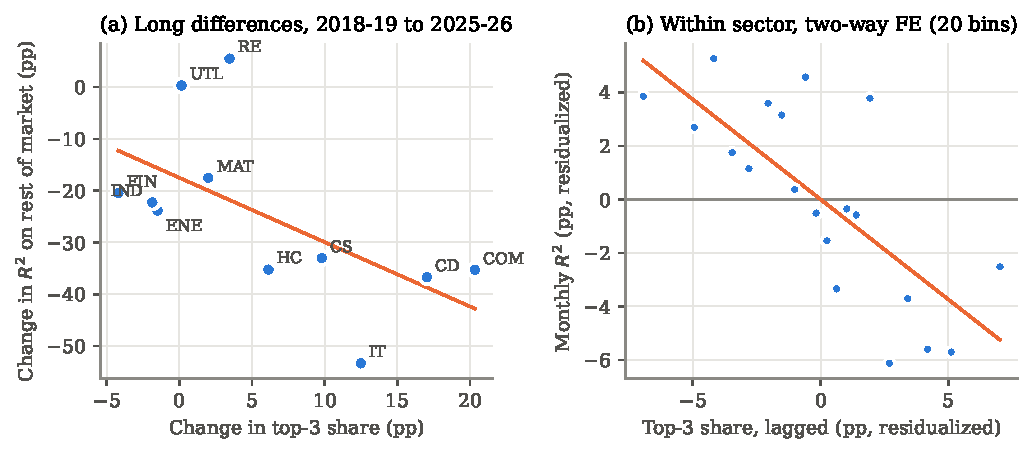
\includegraphics[width=\textwidth]{fig/fig5_concentration_link.pdf}
\caption{Top-three share and co-movement with the rest of the market, uncapped constituent returns. Panel (a): change from October 2018 to September 2019 to the twelve months ending August 2026. Panel (b): binned scatter of lagged top-three share and monthly $R^2$ after removing sector and month fixed effects, log index share, and own volatility; 20 equal-count bins; line is the OLS fit on all observations.}
\label{fig:link}
\end{figure}

\subsection{Granular decomposition}\label{sec:gran}

Figure~\ref{fig:gran}(a) splits each sector's return into its three largest firms and the rest. In 91 of 99 sector-years the top-three component has a lower $R^2$ against the rest of the market than the rest of its own sector. The gap is widest in Consumer Discretionary (41\% against 70\%, averaged over years), Health Care (26\% against 54\%), and Industrials (53\% against 75\%). The top-three component is also the more volatile of the two in 69 of 99 sector-years. The largest firms carry more news of their own.

\begin{figure}[H]
\centering
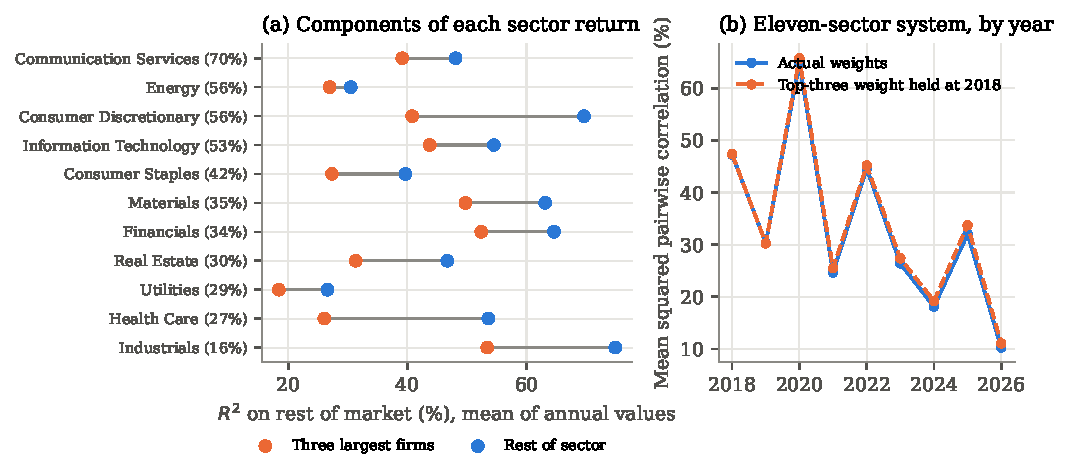
\includegraphics[width=\textwidth]{fig/fig4_granular.pdf}
\caption{Granular decomposition, uncapped constituent returns. Panel (a): mean of annual $R^2$ of each component on the equal-weighted return of the other ten sectors; the average top-three weight is in parentheses. Panel (b): mean squared pairwise correlation among the eleven sector returns by calendar year, with actual weights and with each sector's top-three weight held at its 6 November to 31 December 2018 average.}
\label{fig:gran}
\end{figure}

Table~\ref{tab:cf} measures how much this matters. With each sector's top-three weight held at its late-2018 level, the last-twelve-month $R^2$ of Consumer Discretionary would have been 37.1\% rather than 31.0\%, and the gaps for Materials, Real Estate, and Health Care are between 2.9 and 3.5 points. Those differences are real but small against the fall in co-movement over the sample: Consumer Discretionary's $R^2$ was 77.4\% in the first twelve months. Information Technology runs the other way, because by 2026 its three largest firms co-moved with the market more than the rest of the sector did. For the system, the frozen weights raise average squared correlation over the last twelve months from 10.1\% to 11.0\% and the covariance-based TCI from 48.2\% to 50.0\%; over the first twelve months they leave it at 38.2\%. The composition effect has grown with concentration, from nothing in 2018 and 2019 to between 0.5 and 1.7 points a year from 2020 on (Figure~\ref{fig:gran}(b)).

\begin{table}[H]
\centering
\caption{Counterfactual co-movement with top-three weights held at late-2018 levels}
\label{tab:cf}
\small
\begin{tabular}{lrrrrrr}
\toprule
& \multicolumn{2}{c}{Top-3 weight (\%)} & \multicolumn{3}{c}{$R^2$ on rest of market (\%)} & \\
\cmidrule(lr){2-3}\cmidrule(lr){4-6}
Sector & Late 2018 & Last 12m & First 12m & Last 12m & Counterfactual & Difference \\
\midrule
Communication Services & 61.9 & 81.6 & 64.4 & 17.0 & 18.9 & $-1.9$ \\
Consumer Discretionary & 47.3 & 65.1 & 77.4 & 31.0 & 37.1 & $-6.1$ \\
Consumer Staples & 38.8 & 49.2 & 50.2 & 4.0 & 5.6 & $-1.7$ \\
Energy & 55.7 & 54.3 & 51.9 & 3.1 & 2.7 & 0.4 \\
Financials & 36.0 & 31.0 & 66.6 & 30.3 & 31.3 & $-1.0$ \\
Health Care & 27.9 & 32.4 & 68.0 & 15.8 & 18.8 & $-2.9$ \\
Industrials & 19.1 & 17.4 & 79.8 & 42.7 & 43.5 & $-0.8$ \\
Information Technology & 44.1 & 56.5 & 75.2 & 5.5 & 4.0 & 1.5 \\
Materials & 36.4 & 37.7 & 65.6 & 38.3 & 41.8 & $-3.5$ \\
Real Estate & 27.8 & 31.0 & 27.8 & 26.9 & 30.3 & $-3.4$ \\
Utilities & 27.8 & 27.9 & 8.7 & 9.4 & 10.5 & $-1.1$ \\
\bottomrule
\end{tabular}

\smallskip
\parbox{0.95\textwidth}{\footnotesize Late 2018 is 6 November to 31 December 2018. First 12m is October 2018 to September 2019; last 12m is September 2025 to August 2026. $R^2$ of the uncapped sector return on the equal-weighted return of the other ten sectors. The counterfactual holds the top-three weight at its late-2018 value in every sector and keeps component returns as observed. Difference is actual minus counterfactual.}
\end{table}

%============================================================
\section{Reading the results that run against intuition}\label{sec:disc}
%============================================================

\textbf{Record concentration, record-low connectedness.} The time series invites a simple story: the index concentrated, the sectors drifted apart, so concentration pulled them apart. The decomposition rejects that version of the story. The weight shift toward the largest firms accounts for about one point of a 28-point fall in average squared correlation, and most of the decline happened inside both components. A more promising explanation runs through the firms themselves. Over the last twelve months the top-three components of Communication Services, Consumer Discretionary, and Information Technology have an average pairwise correlation of 0.49, against 0.16 for the rest of those sectors. The same top-three components have an average correlation of 0.08 with the other eight sectors. The market's leading names form a cluster that crosses three GICS sectors, and each of those sector returns mixes the cluster with firms that have little to do with it. The sector partition is losing its grip on how returns actually group, and a connectedness measure built on that partition records the loss as disconnection. Whether index options priced the same shift, through implied correlation, is a natural next test.

\textbf{Why concentrated sectors co-move less.} Two channels predict it. The first is diversification arithmetic. If firm returns are $r_i=\beta_i f + \varepsilon_i$ with similar idiosyncratic variances $\sigma^2_\varepsilon$, a sector's idiosyncratic variance is close to $\text{HHI}\cdot\sigma^2_\varepsilon$, so its $R^2$ on the common factor falls as the Herfindahl index rises. This is the argument of \citet{gabaix2011} applied one level down, and it is strengthened here because the largest firms are also the more volatile and less market-correlated part of the sector. The second channel runs in reverse. Firms become dominant through large returns of their own, so the months in which a sector concentrates are, almost by construction, months of firm-specific news. The counterfactual in Table~\ref{tab:cf} isolates the first channel and finds it modest: Communication Services gained 20 points of top-three weight and lost 1.9 points of $R^2$ to it. The panel coefficient, 0.75 points of $R^2$ per point of top-three share, is several times larger, which is what the second channel would produce.

\textbf{Receivers that are really isolates.} Energy and Utilities are the largest net receivers in Table~\ref{tab:static}, and Information Technology moves from a NET of $+11.4$ in 2019 to $-13.8$ in 2024. With no lag dynamics, a net receiver is simply a sector weakly correlated with the rest. Energy's daily variance is dominated by oil-specific news, and Utilities trade on rates and regulation. Information Technology's $R^2$ against the rest of the market fell from 71\% in 2019 to 24\% in 2024 and 3\% in 2026 on constituent returns. Leading the market's returns is not the same as sharing its shocks.

\textbf{Sectors that reversed together.} In February to June 2020 every sector's lagged return predicted every other sector's with nearly the same negative coefficient as its own. That is the footprint of liquidity, not transmission. Price moves driven by liquidity demand reverse \citep{campbell1993}, and the returns to supplying liquidity rise steeply with the VIX \citep{nagel2012}, which averaged 39.5 in that window and peaked at 82.7 on 16 March 2020. Sector funds are index products, whose growth \citet{baltussen2019} link to negative daily autocorrelation in index returns.

\textbf{Implications.} For portfolio construction, a book diversified across GICS sectors in 2026 holds the same cluster of firms through three sector funds, so diversification measured across sectors overstates diversification across the firms that carry the weight. For connectedness research, three practices follow from this paper: report the covariance-only benchmark next to the full model, report net measures under a scalar normalization, and use randomization inference when regressing filtered connectedness on slow-moving variables.

Two limitations matter most. First, the constituent panel covers 85\% of index members at the start of the sample, because firms acquired and delisted before 2026 cannot be recovered; the missing firms are mostly small, and their absence overstates early concentration, which biases the time trend in concentration toward zero. Second, with eleven sectors the evidence is an association with limited power. It is clear on uncapped returns and weaker on fund returns, and it is not a causal estimate.

%============================================================
\section{Conclusion}
%============================================================

Sectors of the S\&P 500 share shocks within the day but do not forecast each other from one day to the next, so their connectedness is a reading of the correlation matrix. Read that way, the evidence is consistent. Sectors dominated by a few firms co-move less with the rest of the market, because their largest firms carry more news of their own. The weight shift toward those firms is too small, though, to explain why the eleven sectors reached their lowest connectedness of the sample in 2026. That decline points to a market whose main lines of co-movement no longer follow sector boundaries, and measuring connectedness on clusters of firms rather than GICS labels is the obvious next step.

\bigskip
\noindent\textbf{Data availability.} Fund prices, index constituents and share counts are from public sources: Yahoo Finance for prices, share counts and the VIX; Wikipedia's list of S\&P 500 companies for current GICS classifications and addition dates; and a publicly maintained file of historical S\&P 500 membership for removals. The processed data and code that reproduce every table and figure are available from the author on request.

%============================================================
\begin{thebibliography}{99}
\setlength{\itemsep}{2pt}

\bibitem[Antonakakis et~al.(2020)]{antonakakis2020}
Antonakakis, N., Chatziantoniou, I., and Gabauer, D. (2020). Refined measures of dynamic connectedness based on time-varying parameter vector autoregressions. \textit{Journal of Risk and Financial Management}, 13(4), 84.

\bibitem[Baltussen et~al.(2019)]{baltussen2019}
Baltussen, G., van Bekkum, S., and Da, Z. (2019). Indexing and stock market serial dependence around the world. \textit{Journal of Financial Economics}, 132(1), 26-48.

\bibitem[Barun\'ik and K\v{r}ehl\'ik(2018)]{barunik2018}
Barun\'ik, J., and K\v{r}ehl\'ik, T. (2018). Measuring the frequency dynamics of financial connectedness and systemic risk. \textit{Journal of Financial Econometrics}, 16(2), 271-296.

\bibitem[Benjamini and Hochberg(1995)]{benjamini1995}
Benjamini, Y., and Hochberg, Y. (1995). Controlling the false discovery rate: A practical and powerful approach to multiple testing. \textit{Journal of the Royal Statistical Society: Series B}, 57(1), 289-300.

\bibitem[Billio et~al.(2012)]{billio2012}
Billio, M., Getmansky, M., Lo, A. W., and Pelizzon, L. (2012). Econometric measures of connectedness and systemic risk in the finance and insurance sectors. \textit{Journal of Financial Economics}, 104(3), 535-559.

\bibitem[Caloia et~al.(2019)]{caloia2019}
Caloia, F. G., Cipollini, A., and Muzzioli, S. (2019). How do normalization schemes affect net spillovers? A replication of the Diebold and Yilmaz (2012) study. \textit{Energy Economics}, 84, 104536.

\bibitem[Cameron et~al.(2008)]{cameron2008}
Cameron, A. C., Gelbach, J. B., and Miller, D. L. (2008). Bootstrap-based improvements for inference with clustered errors. \textit{Review of Economics and Statistics}, 90(3), 414-427.

\bibitem[Campbell et~al.(1993)]{campbell1993}
Campbell, J. Y., Grossman, S. J., and Wang, J. (1993). Trading volume and serial correlation in stock returns. \textit{Quarterly Journal of Economics}, 108(4), 905-939.

\bibitem[Campbell et~al.(2001)]{campbell2001}
Campbell, J. Y., Lettau, M., Malkiel, B. G., and Xu, Y. (2001). Have individual stocks become more volatile? An empirical exploration of idiosyncratic risk. \textit{Journal of Finance}, 56(1), 1-43.

\bibitem[Campbell and Thompson(2008)]{campbell2008}
Campbell, J. Y., and Thompson, S. B. (2008). Predicting excess stock returns out of sample: Can anything beat the historical average? \textit{Review of Financial Studies}, 21(4), 1509-1531.

\bibitem[Clark and West(2007)]{clark2007}
Clark, T. E., and West, K. D. (2007). Approximately normal tests for equal predictive accuracy in nested models. \textit{Journal of Econometrics}, 138(1), 291-311.

\bibitem[Diebold and Yilmaz(2009)]{diebold2009}
Diebold, F. X., and Yilmaz, K. (2009). Measuring financial asset return and volatility spillovers, with application to global equity markets. \textit{Economic Journal}, 119(534), 158-171.

\bibitem[Diebold and Yilmaz(2012)]{diebold2012}
Diebold, F. X., and Yilmaz, K. (2012). Better to give than to receive: Predictive directional measurement of volatility spillovers. \textit{International Journal of Forecasting}, 28(1), 57-66.

\bibitem[Diebold and Yilmaz(2014)]{diebold2014}
Diebold, F. X., and Yilmaz, K. (2014). On the network topology of variance decompositions: Measuring the connectedness of financial firms. \textit{Journal of Econometrics}, 182(1), 119-134.

\bibitem[Driscoll and Kraay(1998)]{driscoll1998}
Driscoll, J. C., and Kraay, A. C. (1998). Consistent covariance matrix estimation with spatially dependent panel data. \textit{Review of Economics and Statistics}, 80(4), 549-560.

\bibitem[Ferson et~al.(2003)]{ferson2003}
Ferson, W. E., Sarkissian, S., and Simin, T. T. (2003). Spurious regressions in financial economics? \textit{Journal of Finance}, 58(4), 1393-1413.

\bibitem[Gabaix(2011)]{gabaix2011}
Gabaix, X. (2011). The granular origins of aggregate fluctuations. \textit{Econometrica}, 79(3), 733-772.

\bibitem[Grullon et~al.(2019)]{grullon2019}
Grullon, G., Larkin, Y., and Michaely, R. (2019). Are US industries becoming more concentrated? \textit{Review of Finance}, 23(4), 697-743.

\bibitem[Hong et~al.(2007)]{hong2007}
Hong, H., Torous, W., and Valkanov, R. (2007). Do industries lead stock markets? \textit{Journal of Financial Economics}, 83(2), 367-396.

\bibitem[Hou(2007)]{hou2007}
Hou, K. (2007). Industry information diffusion and the lead-lag effect in stock returns. \textit{Review of Financial Studies}, 20(4), 1113-1138.

\bibitem[Koop et~al.(1996)]{koop1996}
Koop, G., Pesaran, M. H., and Potter, S. M. (1996). Impulse response analysis in nonlinear multivariate models. \textit{Journal of Econometrics}, 74(1), 119-147.

\bibitem[Koop and Korobilis(2013)]{koop2013}
Koop, G., and Korobilis, D. (2013). Large time-varying parameter VARs. \textit{Journal of Econometrics}, 177(2), 185-198.

\bibitem[Kwon et~al.(2024)]{kwon2024}
Kwon, S. Y., Ma, Y., and Zimmermann, K. (2024). 100 years of rising corporate concentration. \textit{American Economic Review}, 114(7), 2111-2140.

\bibitem[Lastrapes and Wiesen(2021)]{lastrapes2021}
Lastrapes, W. D., and Wiesen, T. F. P. (2021). The joint spillover index. \textit{Economic Modelling}, 94, 681-691.

\bibitem[Menzly and Ozbas(2010)]{menzly2010}
Menzly, L., and Ozbas, O. (2010). Market segmentation and cross-predictability of returns. \textit{Journal of Finance}, 65(4), 1555-1580.

\bibitem[Nagel(2012)]{nagel2012}
Nagel, S. (2012). Evaporating liquidity. \textit{Review of Financial Studies}, 25(7), 2005-2039.

\bibitem[Parkinson(1980)]{parkinson1980}
Parkinson, M. (1980). The extreme value method for estimating the variance of the rate of return. \textit{Journal of Business}, 53(1), 61-65.

\bibitem[Pesaran and Shin(1998)]{pesaran1998}
Pesaran, M. H., and Shin, Y. (1998). Generalized impulse response analysis in linear multivariate models. \textit{Economics Letters}, 58(1), 17-29.

\bibitem[Rapach et~al.(2019)]{rapach2019}
Rapach, D. E., Strauss, J. K., Tu, J., and Zhou, G. (2019). Industry return predictability: A machine learning approach. \textit{Journal of Financial Data Science}, 1(3), 9-28.

\bibitem[Vilasuso(2001)]{vilasuso2001}
Vilasuso, J. (2001). Causality tests and conditional heteroskedasticity: Monte Carlo evidence. \textit{Journal of Econometrics}, 101(1), 25-35.

\bibitem[Webb(2023)]{webb2023}
Webb, M. D. (2023). Reworking wild bootstrap-based inference for clustered errors. \textit{Canadian Journal of Economics}, 56(3), 839-858.

\bibitem[Young(2019)]{young2019}
Young, A. (2019). Channeling Fisher: Randomization tests and the statistical insignificance of seemingly significant experimental results. \textit{Quarterly Journal of Economics}, 134(2), 557-598.

\end{thebibliography}

\end{document}
